\documentclass[11pt,a4paper]{book}
\usepackage[english,greek]{babel}
\usepackage[utf8x]{inputenc}
\usepackage[noend]{algpseudocode}
\usepackage{algorithm}
\usepackage{amssymb,latexsym,amsmath,ucs,amsthm,setspace,graphicx,fancyvrb,float}
\newtheorem*{lemma}{Λήμμα}
\newcommand{\HRule}{\rule{\linewidth}{0.5mm}}
\newcommand{\defeq}{\overset{\underset{\mathrm{def}}{}}{=}}
\makeatletter
\def\imod#1{\allowbreak\mkern10mu({\operator@font mod}\,\,#1)}
\makeatother
\raggedbottom
\begin{document}

\begin{titlepage}
\begin{center}


\includegraphics[width=0.15\textwidth]{Pyrforos3.png}\\[1cm]
\textsc{\LARGE Εθνικό Μετσόβιο Πολυτεχνείο}\\[1.5cm]

\Large{ 1η Γραπτή Άσκηση }\\[0.5cm]

% Title
\begin{doublespace}
\HRule \\[0.4cm]
{\huge \bfseries
Αλγόριθμοι \& Πολυπλοκότητα
}\\[0.4cm]
\end{doublespace}

\HRule \\[1.5cm]

\begin{minipage}{0.4\textwidth}
\begin{flushleft} \large
\emph{Σπουδαστής:} \\
Διονύσης \textsc{Ζήνδρος} (06601)\\
\textlatin{\textless dionyziz@gmail.com\textgreater}
\end{flushleft}
\end{minipage}
\begin{minipage}{0.4\textwidth}
\begin{flushright} \large
\emph{Διδάσκοντες:} \\
Στάθης \textsc{Ζάχος}\\
Δημήτρης \textsc{Φωτάκης}
\end{flushright}
\end{minipage}

\vfill

{\large 8 Δεκεμβρίου 2011}
\end{center}
\end{titlepage}

\section*{Άσκηση 1}
\subsection*{(α)}

Αρχικά χωρίζουμε τις συναρτήσεις σε πολυωνυμικές και μη πολυωνυμικές και στη συνέχεια ταξινομούμε τις επί μέρους συναρτήσεις. Παρατηρούμε τις εξής χρήσιμες σχέσεις:

\begin{align*}
\log n^3 &\in \Theta( \log n )\\
\log( n! ) &\in \Theta( n \log n )\\
5^{(lg n)} &\in \Theta( n^{\frac{1}{log_5 2}} )\\
(\log n)^{\log n} &\in \Theta( n^{\log \log n} )
\end{align*}

\begin{align*}
\sum_{k=1}^n k^5 \in & O( \sum_{k=1}^n n^5 )\\
= & O( n*n^5 )\\
= & O( n^6 ) \\
\sum_{k=1}^n k^5 \in & \Omega( \sum_{k=1}^n (\frac{n}{2})^5 )\\
= & \Omega( (\frac{n}{2}) * (\frac{n}{2})^5 )\\
= & \Omega( (\frac{n}{2})^6 ) = \Omega( n^6 ) \\
\sum_{k=1}^n k^5 \in & \Theta( n^6 )
\end{align*}

\begin{align*}
\sqrt{n!} \in & O( \sqrt{ n^n } )\\
= & O( n^{\frac{n}{2}} )\\
\sqrt{n!} \in & \Omega( \sqrt{ ( \frac{n}{2} )^{ \frac{n}{2} } } ) \\
= & \Omega( (\frac{n}{2})^{\frac{n}{4}} )
\end{align*}

Με βάση αυτά καταλήγουμε στην παρακάτω διάταξη:

\begin{align*}
\Theta( \log n^3 ) &\subset& \Theta( \sqrt n \log^{50} n ) &\subset& \Theta( \frac{n}{\log \log n} )\subset \\
\Theta(\log( n! )) &\subset& \Theta( n \log^{10} n ) &\subset& \Theta( n^{1.01} )\subset \\
\Theta( 5^{(lg n)} ) &\subset& \Theta( \sum_{k=1}^n k^5 ) &\subset& \Theta( (\log n)^{\log n} ) = \\
\Theta( n^{\log \log n} ) &\subset& \Theta( 2^{(\lg n)^4} ) &\subset& \Theta( (\log n)^{\sqrt n} ) \subset\\
\Theta( e^{\frac{n}{\ln n}} ) &\subset& \Theta( n {3^n} ) &\subset& \Theta( 2^{2n} ) \subset\\
\Theta( \sqrt{n!} )
\end{align*}

\subsection*{(β)}

\begin{enumerate}
\item Αφού $n \log n \in \Omega( n^{log_7 5 + \epsilon} )$ άρα από το \textlatin{Master Theorem} θα είναι: 
\[ T \in \Theta( n \log n )\]
\item Αφού $\frac{n}{log^2 n} \in \Omega( n^{log_5 4 + \epsilon} )$ άρα από το \textlatin{Master Theorem} θα είναι:
\[ T \in \Theta( \frac{n}{log^2 n} ) \]
\item Θα δείξω ότι $T \in O( n )$. Αρκεί να δείξω ότι $\forall n \in \mathbb{N}: T( n ) \leq 21n$. Πράγματι, με ισχυρή επαγωγή έχουμε:
\[
T( 1 ) = 1 \leq 21
\]

Έστω $\forall n < n_0: T(n) \leq 21n$. Τότε:

\begin{align*}
T( n_0 ) & = T( \frac{n_0}{3} ) + 3T( \frac{n_0}{7} ) + n_0 \\
         & \leq 21 \frac{n_0}{3} + 21 * 3 * \frac{n_0}{7} + n_0 \\
         & = 7 n_0 + 9 n_0 + n_0 \leq 21 n_0.
\end{align*}

Άρα $T \in O( n )$.

Θα δείξω τώρα ότι $T \in \Omega( n )$. Αρκεί να δείξω ότι $\forall n \in \mathbb{N}: T( n ) \geq n$. Πράγματι, με ισχυρή επαγωγή έχουμε:
\[
T( 1 ) = 1 \geq 1
\]

Έστω $\forall n < n_0: T( n ) \geq n$. Τότε:

\begin{align*}
T( n_0 ) & = T( \frac{n_0}{3} ) + 3T( \frac{n_0}{7} ) + n_0\\
& \geq \frac{n_0}{3} + 3 \frac{n_0}{7} + n_0\\
& \geq n_0
\end{align*}

Άρα $T \in \Omega( n )$ και συνεπώς $T \in \Theta( n )$.

\item Αφού $n \in \Theta( n^{\log_6 6} ) = \Theta( n )$ άρα από το \textlatin{Master Theorem} θα είναι $T \in \Theta( n \log n )$.
\item Από το δέντρο της αναδρομής έχουμε τα φράγματα $T \in O( n \log_{\frac{3}{2}}n )$ και $T \in \Omega( n \log_3 n )$ και άρα $T \in \Theta( n \log n )$.
\item Αφού $n^3 \log^2 n \in \Omega( n^{2 + \epsilon} ) $ άρα από το \textlatin{Master Theorem} θα είναι $T \in \Theta( n^3 \log^2 n )$ 
\item Θα είναι:
\begin{align*}
T( n ) & = \sum_{i=1}^{\lg\lg n} \lg\lg 2^{2^i}\\
       & = \sum_{i=1}^{\lg\lg n} \lg 2^i\\
       & = \sum_{i=1}^{\lg\lg n} i\\
       & \in \Theta( ( \lg\lg n )^2 )\\
\end{align*}
       
\item Έχουμε:

\begin{align*}
            T( n ) &= T( n - 3 ) + \log n \\
\Rightarrow T( n ) &= \sum_{i = 0}^{\frac{n}{3} - \frac{1}{3}} \log( 3i + 1 )\\
                   &= \log( \prod_{i = 0}^{\frac{n}{3} - \frac{1}{3}} (3i + 1) )
\end{align*}

Συνεπώς είναι:

\begin{align*}
T( n ) \in & O( \log( n! ) )\\
         = & O( n \log n )
\end{align*}

Επιπλέον είναι:

\begin{align*}
T( n ) \in & \Omega( \log( \frac{n}{3}! ) ) \\
         = & \Omega( \log (( \frac{n}{6} )^{\frac{n}{6}}) ) \\
         = & \Omega( n \log n )
\end{align*}

Άρα $T( n ) \in \Theta( n \log n )$.
\end{enumerate}

\section*{Άσκηση 2}
Χρησιμοποιούμε ένα \textlatin{AVL} δέντρο για να κρατάμε τα στοιχεία μας. Ξεκινώντας με ένα άδειο δέντρο εισάγουμε όλα τα στοιχεία προσέχοντας να μην εισάγουμε πολλαπλά ταυτόσημα στοιχεία. Αντίθετα, κατά την εισαγωγή ενός στοιχείου που υπάρχει ήδη, αυξάνουμε ένα μετρητή που δείχνει το πλήθος των εμφανίσεών του. Τέλος, εξάγουμε τα στοιχεία σε αύξουσα σειρά εισάγοντας το κατάλληλο πλήθος στον πίνακα που θα επιστρέψουμε. Καθώς το δέντρο θα περιέχει κάθε στιγμή το πολύ $\lg n$ στοιχεία, οι λειτουργίες εισαγωγής στοιχείου και εξαγωγής ελαχίστου θα είναι $O( \lg \lg n )$.

\selectlanguage{english}
\begin{algorithm}[H]
\caption{\textgreek{Άσκηση 2}}
\begin{algorithmic}[1]
\Procedure{FastRepeatedSort}{$A, N$}
    \State $t \gets \Call{EmptyBalancingTree}$
    \For{$i \gets 1$ to $N$}
        \State $item \gets \Call{TreeFind}{t, A[ i ]}$
        \If{$item \neq \bot$}
            \State $item.count \gets item.count + 1$
        \Else
            \State $\Call{TreeInsert}{t, key: A[ i ], count: 1}$
        \EndIf
    \EndFor
    \State $j \gets 1$
    \While{$\lnot \Call{Empty}{t}$}
        \State $item \gets \Call{ExtractMin}{t}$
        \For{$i \gets 1$ to $item.count$}
            \State $A[ j ] \gets item.key$
            \State $j \gets j + 1$
        \EndFor
    \EndWhile
\EndProcedure
\end{algorithmic}
\end{algorithm}
\selectlanguage{greek}

Το κάτω φράγμα στο χρόνο εκτέλεσης του συγκριτικού αλγορίθμου δεν ισχύει καθώς εισάγουμε μία υπόθεση για την κατανομή των στοιχείων με αποτέλεσμα να μπορούμε έτσι να μειώσουμε το πλήθος των πιθανών διατάξεων.

\section*{Άσκηση 3}

\subsection*{(α)}
Αρχικά εντοπίζουμε ένα άνω φράγμα για το πλήθος των στοιχείων του πίνακά μας εξετάζοντας αλλεπάλληλες δυνάμεις του 2. Αυτό επιτυγχάνεται σε χρόνο $\Theta( \log n )$. Στη συνέχεια χρησιμοποιούμε απλή δυαδική αναζήτηση για να εντοπίσουμε αν υπάρχει το εν λόγω στοιχείο σε χρόνο $\Theta( \log \lceil 2^{\log n} \rceil ) = \Theta( \log n )$.

\selectlanguage{english}
\begin{algorithm}[H]
\caption{\textgreek{Άσκηση 3(α)}}
\begin{algorithmic}[1]
\Procedure{SizeUpperBound}{$A$}
    \State $high \gets 1$
    \While{$A[ high ] \neq \infty$}
        \State $high \gets 2high$
    \EndWhile
    \State \Return $high$
\EndProcedure

\Require $sorted(A)$
\Procedure{BinarySearch}{$A, key, low, high$}
    \If{$low \geq high$}
    	\State \Return $\bot$
    \EndIf
    \State $mid \gets \lfloor \frac{low + high}{2} \rfloor$
    \If{$key = A[ mid ]$}
        \State \Return $mid$
    \EndIf
    \If{$key < A[ mid ]$}
        \State \Return \Call{BinarySearch}{$A, key, low, mid$}
    \EndIf
    \If{$key > A[ mid ]$}
        \State \Return \Call{BinarySearch}{$A, key, mid + 1, high$}
	\EndIf
\EndProcedure

\Require $sorted(A)$
\Procedure{Find}{$A, key$}
	\State $N \gets \Call{SizeUpperBound}{A}$
    \State \Return 
    	\Call{BinarySearch}{$A, key, 1, N$}
\EndProcedure
\end{algorithmic}
\end{algorithm}
\selectlanguage{greek}
    
\subsection*{(β)}
Ξεκινάμε με δύο τμήματα των πινάκων $A$ και $B$ που περιέχουν σίγουρα το $k$-οστό στοιχείο. Αυτό σίγουρα θα βρίσκεται στα πρώτα $k$ στοιχεία ενός εκ των δύο. Κρατάμε λοιπόν τα $k$ πρώτα στοιχεια του $A$ και τα $k$ πρώτα στοιχεία του $B$. Στη συνέχεια, διαλέγουμε το μεσαίο στοιχείο των δύο τμηματων τα οποία και συγκρίνουμε. Χρησιμοποιώντας αυτή τη σύγκριση μαζί με την μεταβατικότητα της σύγκρισης και το γεγονός ότι τα δύο τμήματα είναι ταξινομημένα, απορρίπτουμε τον μισό από τα δύο τμήματα. Συνεχίζοντας αυτή τη διαδικασία αναδρομικά, κάποια στιγμή καταλήγουμε στην περίπτωση όπου τα τμήματά μας έχουν λιγότερα από $k$ στοιχεία, και συνεπώς το στοιχείο που αναζητούμε βρίσκεται στο μέρος που πρόκειται να αφαιρεθεί. Καθώς το μέρος αυτό είναι ταξινομημένο, ξέρουμε άμεσα τη θέση του στοιχείου που μας ενδιαφέρει.

Η λύση αυτή χρησιμοποιεί τη μέθοδο ((Διαίρει και εξειδίκευσε)), καθώς κάθε φορά αφαιρεί το μισό ενός από τα δύο τμήματα που μένουν να εξετάσουμε. Έτσι η πολυπλοκότητά της είναι $\Theta( \log k )$.

\selectlanguage{english}
\begin{algorithm}[H]
\caption{\textgreek{Άσκηση 3(β)}}
\begin{algorithmic}[1]
\Require $sorted(A[l_A \dots l_A + k]), sorted(B[l_B \dots l_B + k])$
\Procedure{$K^{th}Element$}{$A, l_A, B, l_B, k$}
	\State $m_A \gets l_A + \lfloor \frac{k - 1}{2} \rfloor$
	\State $m_B \gets l_B + \lfloor \frac{k - 1}{2} \rfloor$
    \If{$k = 1$}
        \State \Return $\min( A[ l_A ], B[ l_B ] )$
    \EndIf
    \State $k \gets \lfloor \frac{k}{2} \rfloor$
    \If{$A[ m_A ] < B[ m_B ]$}
        \State \Return \Call{$K^{th}Element$}{$A, m_A + 1, B, l_B, k$}
    \EndIf
    \State \Return \Call{$K^{th}Element$}{$A, l_A, B, m_B + 1, k$}
\EndProcedure
\Procedure{$K^{th}$}{$A, B, N, k$}
	\State $k \gets \min(N, k)$
	\State \Return \Call{$K^{th}Element$}{$A, 1, B, 1, k$}
\EndProcedure
\end{algorithmic}
\end{algorithm}

\selectlanguage{greek}
        
\section*{Άσκηση 4}
Παρατηρούμε ότι το τεύχος που λείπει θα πρέπει να διαφέρει σε τουλάχιστον ένα \textlatin{bit} από κάθε τεύχος που έχουμε στην κατοχή μας. Ξεκινάμε βρίσκοντας το πρώτο \textlatin{bit} του \textlatin{comicbook} που λείπει. Αυτό γίνεται ευκολα κάνοντας \textlatin{xor} στο πρώτο \textlatin{bit} των τευχών που έχουμε, δηλαδή με $n - 1$ ερωτήσεις. Στη συνέχεια, γνωρίζουμε ότι τα τεύχη που έχουν διαφορετικό το πρώτο \textlatin{bit} είναι σίγουρα διάφορα από το τεύχος που λείπει. Συνεπώς, απομένει να ελέγξουμε τα τεύχη που έχουν ίδιο το πρώτο \textlatin{bit}. Αυτά είναι $\frac{n}{2} - 1$ σε πλήθος. Στη συνέχεια μπορούμε να βρούμε το δεύτερο \textlatin{bit} και να διαγράψουμε πάλι τα μισά τεύχη που διαφέρουν, συνεχίζοντας έτσι τη διαδικασία έως ότου γνωρίζουμε την τιμή όλων των \textlatin{bits}. Καθώς κάθε φορά που μαθαίνουμε ένα \textlatin{bit} αφαιρούμε τα μισά τεύχη που γνωρίζουμε ότι διαφέρουν, το πλήθος των ερωτήσεων δεν θα ξεπεράσει ποτέ το $n + \frac{n}{2} + \frac{n}{4} + \dots = 2n$.

\selectlanguage{english}
\begin{algorithm}[H]
\caption{\textgreek{Άσκηση 4}}
\begin{algorithmic}[1]
\Procedure{MissingComicbook}{$n$}
    \State $candidates \gets \{ x: 1 \leq x \leq n \}$
    \State $result \gets 0$
    \For{$j \gets \log n$ downto $2$}
        \State $x \gets 0$
        \State $candidates_0 \gets \{\}$
        \State $candidates_1 \gets \{\}$
        \ForAll{$i \in candidates$}
            \If{$ask( i, j ) = 1$}
                \State $candidates_1 \gets candidates_1 \cup \{ i \}$
                \State $x \gets 1 - x$
            \Else
                \State $candidates_0 \gets candidates_0 \cup \{ i \}$
            \EndIf
        \EndFor
        \If{$x = 1$}
            \State $candidates \gets candidates \setminus candidates_0$
            \State $result \gets result + 2 ^ j$
        \Else
            \State $candidates \gets candidates \setminus candidates_1$
        \EndIf
    \EndFor
    \State $result \gets result + ask( \bigcup candidates, 1 )$\footnote{Test}
    \State \Return $result$
\EndProcedure
\end{algorithmic}
\end{algorithm}
\selectlanguage{greek}
\footnotetext{Ο τελεστής $\bigcup$ εφαρμοσμένος σε μονοσύνολο επιστρέφει το μοναδικό στοιχείο του μονοσυνόλου.}

\section*{Άσκηση 5}
Διασχίζουμε τις πολυκατοικίες από τα ανατολικά προς τα δυτικά. Κρατούμε κάθε στιγμή μία στοίβα που περιέχει ταξινομημένες σε σειρά αύξουσων υψών τις σφαίρες που κινούνται στον αέρα στη θέση που βρισκόμαστε. Φτάνοντας σε μία πολυκατοικία, ελέγχουμε το πρώτο και μικρότερο στοιχείο της στοίβας για να δούμε αν πρόκειται να υπάρξει κάποια σύγκρουση. Αν ναι, τότε ενημερώνουμε τον πίνακα Β αφού πλέον γνωρίζουμε ότι η εναέρια σφαίρα χτύπησε την πολυκατοικία που εξετάζουμε. Συνεχίζουμε με τον ίδιο τρόπο έως ότου η στοίβα να αδειάσει ή μέχρι να βρούμε κάποια σφαίρα που βρίσκεται σε μεγαλύτερο ύψος από την πολυκατοικία που εξετάζουμε. Στη συνέχεια προσθέτουμε στην αρχή της στοίβας την σφαίρα που φεύγει από την πολυκατοικία που εξετάζουμε. Η στοίβα υποχρεωτικά θα παραμείνει ταξινομημένη καθώς το πρώτο της στοιχείο πριν την εισαγωγή είναι μεγαλύτερο από το στοιχείο που πρόκειται να εισαχθεί.

\begin{figure}
	\caption{Ο αλγόριθμος 5 για $j = 4$ πριν την εσωτερική επανάληψη}
	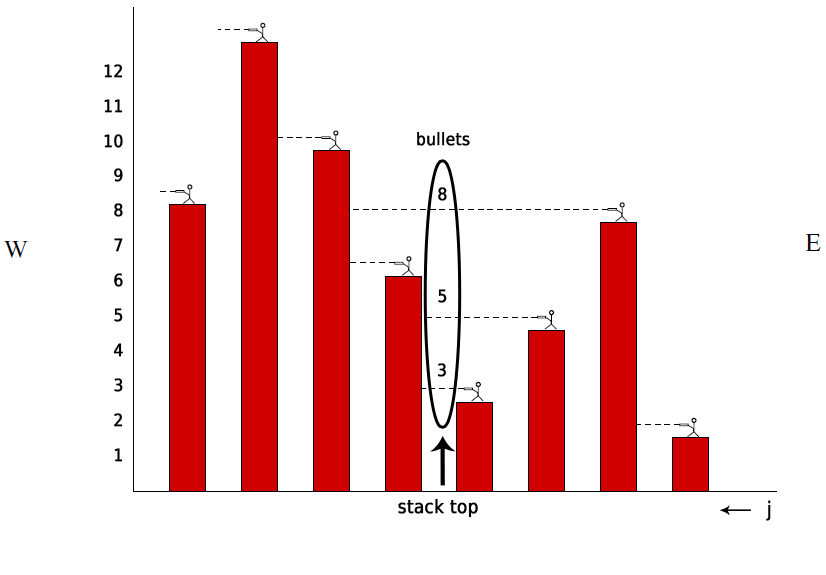
\includegraphics[width=1\textwidth]{5.png}
\end{figure}

Ο αλγόριθμος είναι γραμμικός διότι η συνάρτηση \textlatin{POP} τρέχει μία φορά για κάθε σφαίρα το πλήθος των οποίων είναι $N$. Επιπλέον, γίνεται ένα \textlatin{POP} για κάθε επανάληψη της εσωτερικής \textlatin{while} πέρα από την πρώτη επανάληψη, συνεπώς το πλήθος των επαναλήψεων είναι καθολικά γραμμικά φραγμένο.

\selectlanguage{english}
\begin{algorithm}[H]
\caption{\textgreek{Άσκηση 5}}
\begin{algorithmic}[1]
\Procedure{buildings}{$A, N$}
    \State $B \gets [\ ]$
   	\For {$i \gets N$ downto $1$}
   		\State $B[ i ] \gets 0$
   	\EndFor
    \State $bullets \gets \Call{EmptyStack}$
    \For {$i \gets N$ downto $1$}
        \While {$\lnot \Call{Empty}{bullets}$}
            \State $bullet \gets \Call{Top}{bullets}$
            \If {$A[ bullet ] < A[ i ]$}
                \State $B[ bullet ] \gets i$
                \State $\Call{pop}{bullets}$
            \Else
                \State $break$
            \EndIf
        \EndWhile
        \State $\Call{Push}{bullets, i}$
    \EndFor
    \State \Return $B$
\EndProcedure
\end{algorithmic}
\end{algorithm}

\selectlanguage{greek}

\end{document}
